%
% anfangrand.tex
%
% (c) 2020 Prof Dr Andreas Müller, Hochschule Rapperswil
%
\begin{frame}
\frametitle{Anfangs- und Randwertprobleme}
\vspace{-10pt}
\begin{columns}[t]
\begin{column}{0.48\hsize}
\begin{block}{Anfangswertproblem}
\vspace{-10pt}
\begin{align*}
\frac{d}{dx} \vec{y} &= F(x,\vec{y})\\
\uncover<2->{{\color{blue}\vec{y}(0)}}&\uncover<2->{{\color{blue}=\vec{g}}}
\end{align*}
\end{block}
\end{column}
\begin{column}{0.48\hsize}
\begin{block}{Randwertproblem}
\vspace{-10pt}
\begin{align*}
\frac{d}{dx} \vec{y} &= F(x,\vec{y})\\
\uncover<4->{{\color{blue}y_0(a)}}&\uncover<4->{{\color{blue}=g_0}}\\
\uncover<4->{{\color{blue}y_0(b)}}&\uncover<4->{{\color{blue}=h_0}}
\end{align*}
\end{block}
\end{column}
\end{columns}
\vspace{-15pt}
\begin{columns}[t]
\begin{column}{0.48\hsize}
\begin{center}
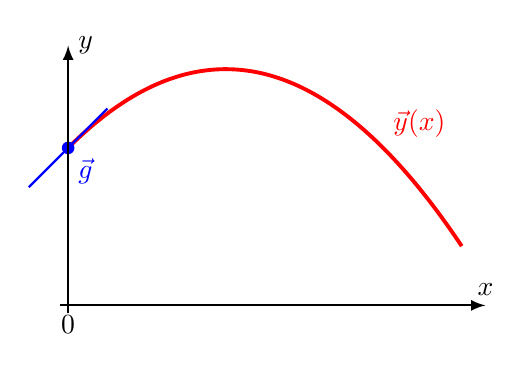
\begin{tikzpicture}[>=latex,thick]
\uncover<3->{
\draw[color=red,line width=1.4pt]
	plot[domain=0:5,samples=100]
		({\x},{3-0.25*(\x-2)*(\x-2)});
\node[color=red] at (4,2) [above right] {$\vec{y}(x)$};
}
\uncover<2->{
\fill[color=blue] (0,2) circle[radius=0.08];
\draw[color=blue] (-0.5,{2-0.5*tan(45)})--(0.5,{2+0.5*tan(45)});
\node[color=blue] at (0,2) [below right] {$\vec{g}$};
}
\draw[->] (-0.1,0)--(5.3,0) coordinate[label={$x$}];
\draw[->] (0,-0.1)--(0,3.3) coordinate[label={right:$y$}];
\node at (0,0) [below] {$0$};
\end{tikzpicture}
\end{center}
\end{column}
\begin{column}{0.48\hsize}
\begin{center}
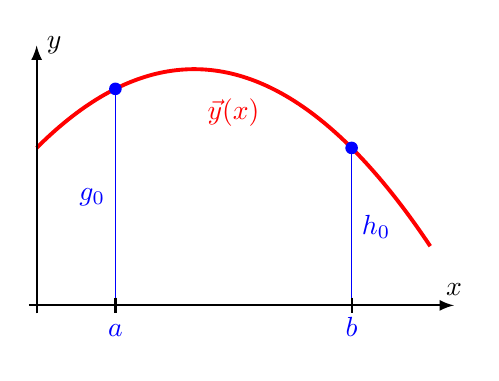
\begin{tikzpicture}[>=latex,thick]
\uncover<5->{
\draw[color=red,line width=1.4pt]
	plot[domain=0:5,samples=100]
		({\x},{3-0.25*(\x-2)*(\x-2)});
\node[color=red] at (2.5,2.75) [below] {$\vec{y}(x)$};
}


\draw[->] (-0.1,0)--(5.3,0) coordinate[label={$x$}];
\draw[->] (0,-0.1)--(0,3.3) coordinate[label={right:$y$}];
\uncover<4->{
\fill[color=blue] (1,2.75) circle[radius=0.08];
\fill[color=blue] (4,2) circle[radius=0.08];
\draw[color=blue,line width=0.5pt] (1,0)--(1,2.75);
\node[color=blue] at (1,1.375) [left] {$g_0$};
\draw[color=blue,line width=0.5pt] (4,0)--(4,2);
\node[color=blue] at (4,1) [right] {$h_0$};
\draw (1,0.1)--(1,-0.1);
\node[color=blue] at (1,0) [below] {$a\mathstrut$};
\draw (4,0.1)--(4,-0.1);
\node[color=blue] at (4,0) [below] {$b\mathstrut$};
}
\end{tikzpicture}
\end{center}
\end{column}
\end{columns}

\end{frame}
